As the S\&C platform will be entirely hosted using Amazon Web Services (AWS), it will utilize a three-layer architecture by design. This architecture consists of the presentation layer for the user interface and interaction, the application layer for data processing, and finally, the database layer where all application data will be stored. The choice of AWS and this architecture came from the ease of deployment, as AWS provides a ready-made solution for this type of application.

\begin{figure}[h]
    \centering
    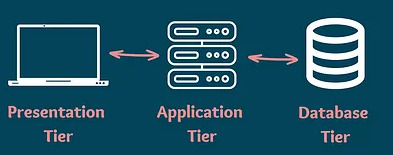
\includegraphics[width=1\linewidth]{DD-Latex//assets/Three tier.jpg}
    \caption{Three tier architecture \cite{MToC_2023}}
    \label{fig:enter-label}
\end{figure}

\subsubsection{Distributed view} 
Figure 2 presents the distributed view of the system, showcasing its function and interaction with other elements. As noted, the system will be hosted on AWS, which utilizes containerization and Kubernetes, allowing the system to scale as needed. Figure 2 depicts a hypothetical example of 27 instances of the service running across three servers and their interactions.
\newpage
\begin{figure}[h]
    \centering
    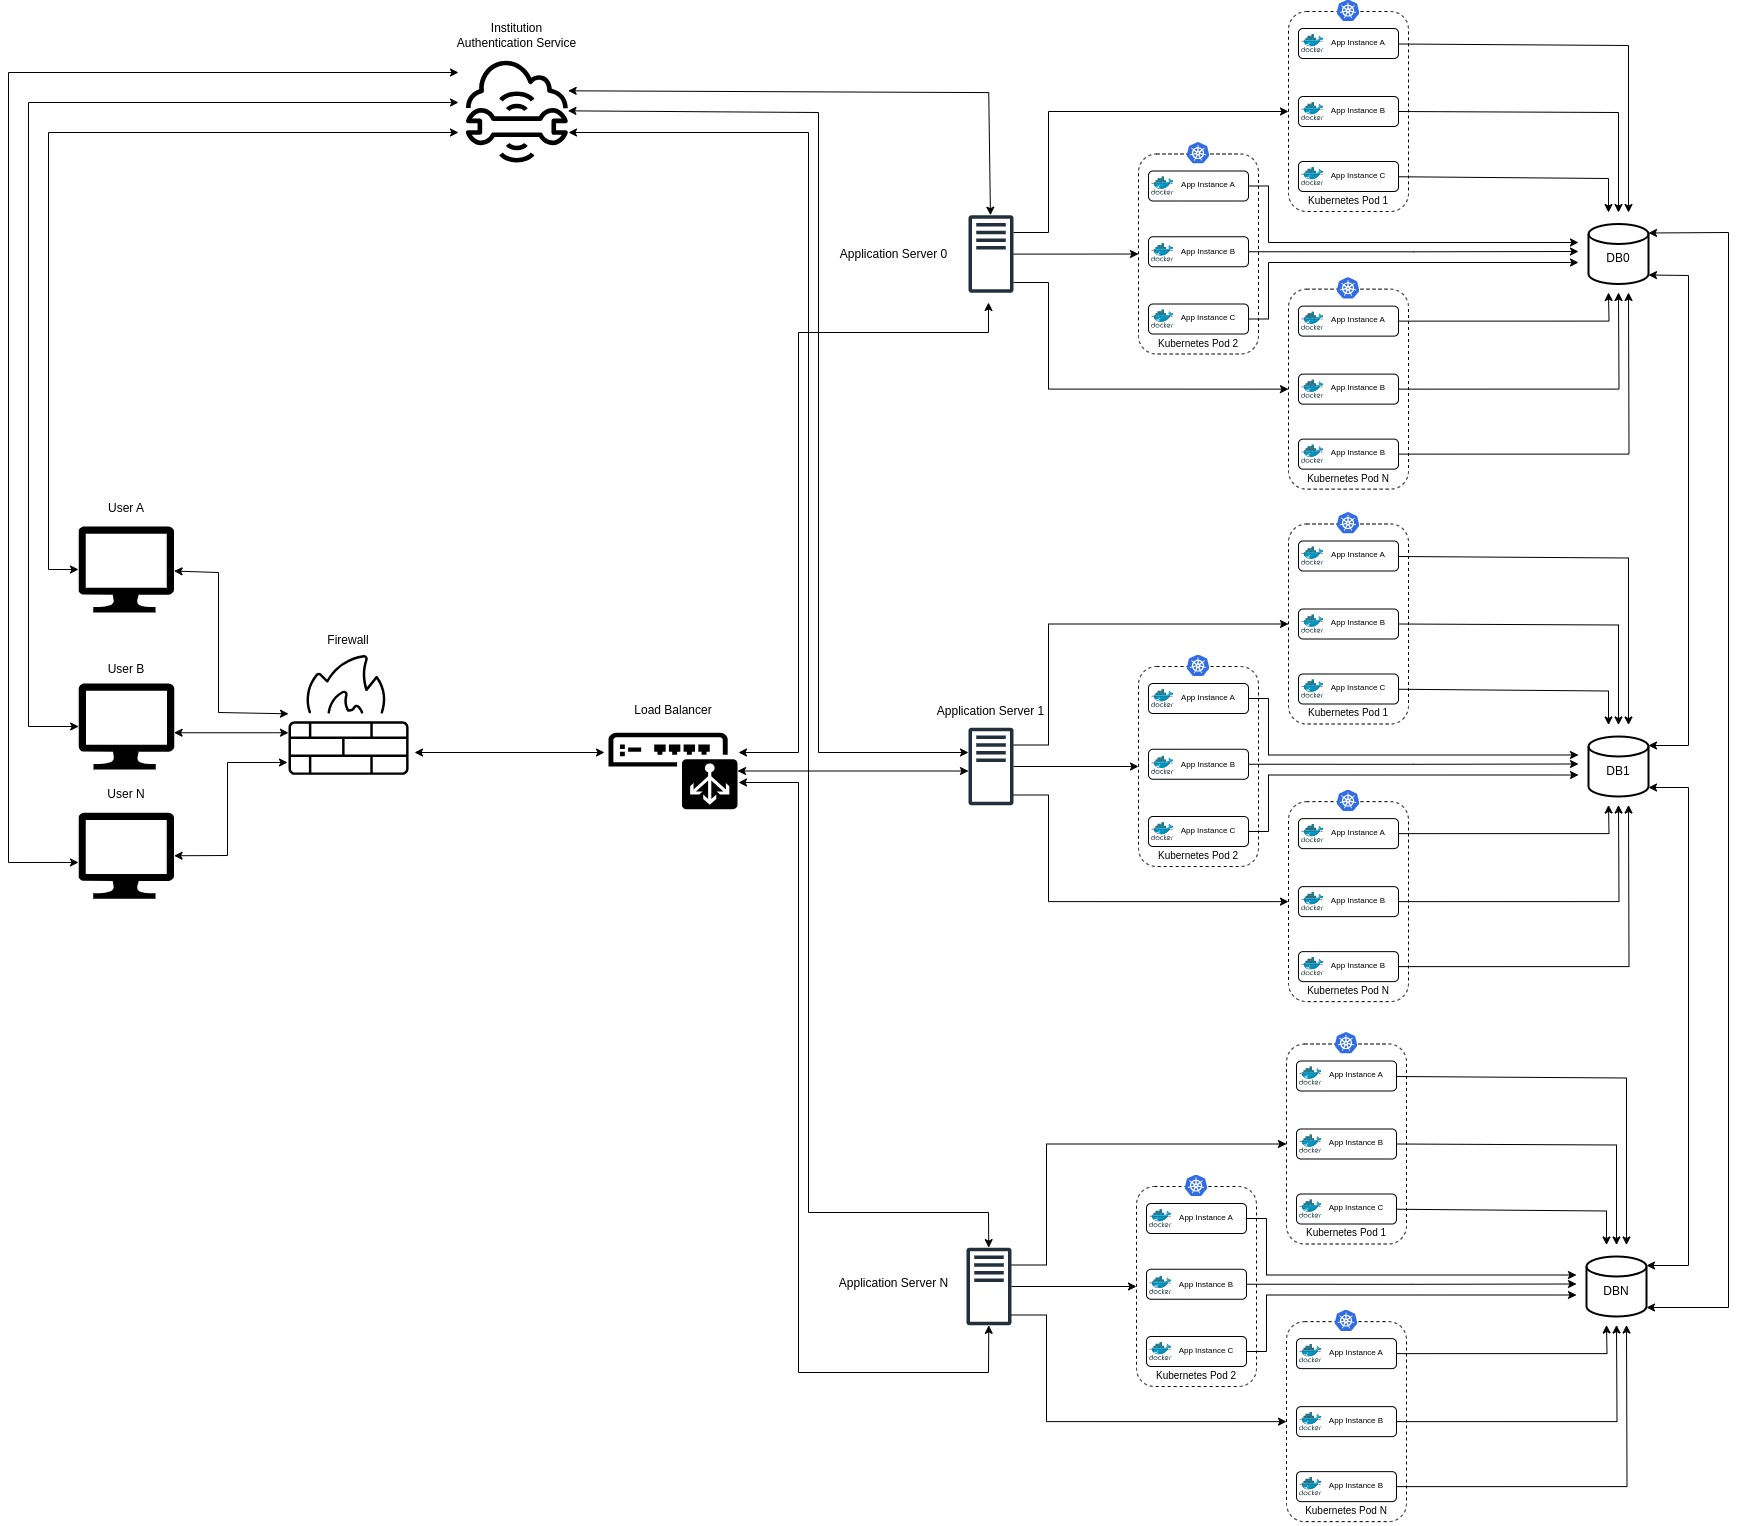
\includegraphics[width=1\linewidth]{DD-Latex//assets//Distributed View/Distributed View.jpg}
    \caption{Distributed view}
    \label{fig:enter-label}
\end{figure}

